\subsection{The one separable group: pups' Isolation calls}\label{sec:iso}
This group was found exploratorily in the discovery sample, and the supervised tests below are also exploratory, blocked by bat, channel, treatment and age; the pre-specified validation in held-out files is reported in Section~\ref{sec:repl}.

\paragraph{Exploratory discovery.} The standard UMAP--HDBSCAN pipeline on 12,000 voiced files returned two clusters at minimum sizes 100 and 300, covering 99.6\% of files: a large one (93.2\%) and a small one of 770 files (6.4\%; Fig.~\ref{fig:iso7}A,B). The small cluster was stable under resampling of bats (Jaccard 0.975, range 0.959--0.993 over 8 bootstraps) and under 15 and 100 UMAP neighbours, spanned 30 of 42 emitter groups and several channels (the most common channel held 38\% of it, against 36\% of the large cluster), and was not a duration or silence group (voiced-duration AUC 0.54, silence AUC 0.47; median 1 voiced segment against 2). It was 86\% Isolation-context files (662/770) and contained 83\% of the Isolation files, which are 6.7\% of the sample; among positive-coded pups, 87.8\% of Isolation files fell in the cluster against only 2.0\% of the same pups' files from other contexts and 0.4\% of adults' (non-Isolation) files (NMI 0.651 against a within-channel$\times$month permutation null of 0.062, maximum 0.083; 0 of 1,000). On an axis learned from other bats the two groups were separated by $d'=7.0$ (range 5.7--8.3). Cluster counts and noise shares of HDBSCAN solutions are, however, fragile statistics: null datasets (Gaussian-copula, session-mean, curved-continuum, skewed) fragmented into 2--13 clusters with 38--77\% noise, but the real data with the small cluster removed also fragmented (15 clusters, 48\% noise at minimum size 100, three at size 30; Fig.~\ref{fig:iso7}B), so we do not treat the contrast with the nulls as evidence by itself. Blind recovery was also representation-dependent: on the whole-span features four clusters resulted, one of which (675 files) was 91\% Isolation-context with 77\% of the Isolation files, the others following recording channel (Cram\'er's $V$ of the partition with channel 0.64); on syllable shapes a 464-syllable cluster (3.9\%) was 78\% Isolation-context (82\% of Isolation syllables); on voiced MFCC statistics only a 0.9\% single-channel micro-cluster appeared. The evidence for the group therefore rests on the tests that follow and on the algorithm comparison above, not on the unsupervised discovery alone.

\begin{figure}[!t]\centering
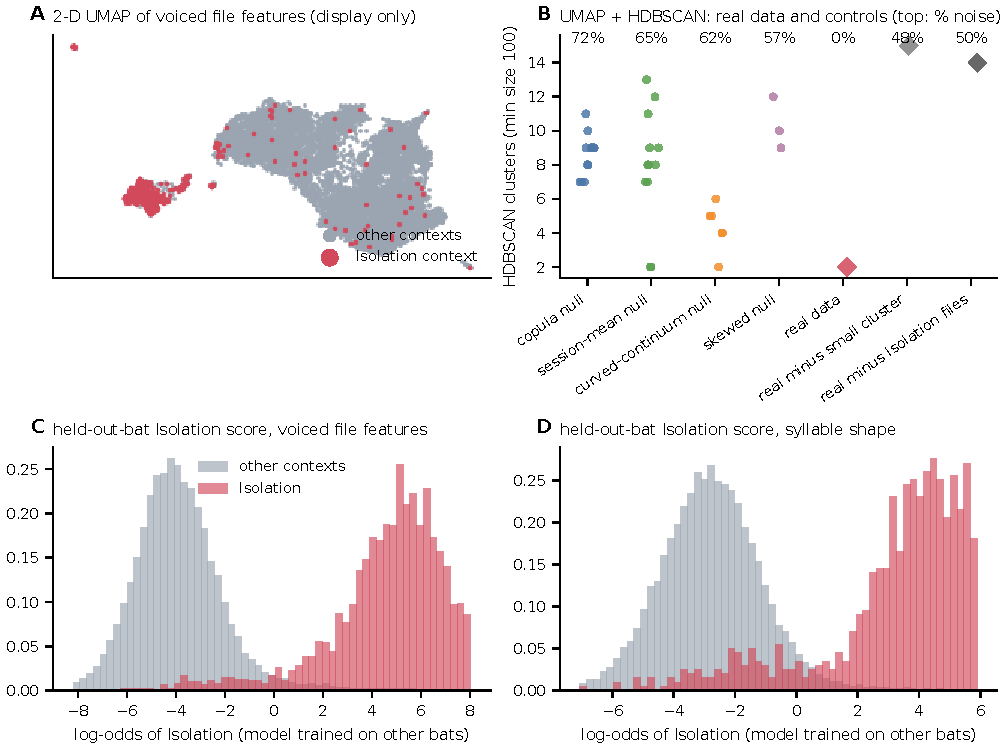
\includegraphics{fig4_v4.pdf}
\caption{(A) 2-D UMAP of 12,000 voiced file feature vectors with Isolation-context files highlighted (display only). (B) Number of HDBSCAN clusters (minimum size 100) for the real data, null datasets without discrete structure (12 Gaussian-copula, 12 session-mean, 6 curved-continuum, 3 skewed) and the real data with the small cluster or all Isolation files removed; the number above each group is the mean share of points labelled noise. (C, D) Held-out-bat score (log-odds of Isolation from a model trained on other bats) for voiced file features (C) and syllable shapes (D).}\label{fig:iso7}
\end{figure}

\paragraph{Supervised separability (discovery sample).} Predicting Isolation from the voiced features with folds blocked by bat gave AUC 0.984 (95\% CI \ci{0.979}{0.991}; voiced MFCCs 0.984), $d'=4.5$, with only 3.2\% of non-Isolation files scoring above the 5th percentile of Isolation files. The pooled out-of-fold score was bimodal (dip $p=3\times10^{-4}$) while the scores of non-Isolation files alone were unimodal ($p=0.996$): the Isolation files formed a separate mode, not the tail of the others (Fig.~\ref{fig:iso7}C). The result held within pups only (AUC 0.982, \ci{0.969}{0.990}; the same 20 pups' other contexts), within channel$\times$month strata (weighted mean 0.90), without the unknown-emitter group that supplies 57\% of Isolation files (0.984), for each of 15 identified pups from a model blind to that pup (median 0.97, range 0.83--1.00), with each channel or treatment held out in turn (0.983 over 8 channels; 0.986 over 6 treatments) and within pup-age windows from day 40 (0.70 at 40--60 days, 0.93 at 60--90, 0.97 at 90--150), although pups younger than 40 days contribute almost only Isolation files (183 against 4), so age and context cannot be separated there. At the syllable level the separation was weaker but clear (AUC 0.956, \ci{0.944}{0.974}; $d'=3.7$; 30--33\% of non-Isolation syllables scored above the 5th percentile of Isolation; Fig.~\ref{fig:iso7}D), and AVES embeddings separated the group no better than handcrafted features (AUC 0.93--0.95 against 0.94--0.97 on 1,000 files). All variants are in Supplement Table~S4; the unsupervised tests could not be expected to find a group this small (Fig.~\ref{fig:power}), and a forced two-way split of all files is dominated by other variation.

\subsection{Pre-specified validation in every remaining annotated file}\label{sec:repl}
Criteria for the two out-of-sample sets were written to the analysis log before any of their files was analysed, and no analysis choice used these files. They come from the same corpus and share all of their positive-coded bats and channels with the discovery sample (Supplement Table~S5b), so they test over-fitting to the discovery recordings, not generalisation to other colonies. All three criteria were met in both sets (Supplement Table~S5; Supplement Fig.~S6b). In the 12,000-file replication sample the model trained on the discovery files separated Isolation from all other contexts with AUC 0.988 (\ci{0.978}{0.992}; $d'=5.1$; pups only 0.985), and UMAP--HDBSCAN fitted on the new files alone returned two clusters (94.2\% and 5.8\%; no noise) of which the small one held 695 files from 24 emitter groups and was 90.1\% Isolation-context. In the completion sample (all 33,557 remaining annotated files; 2,089 Isolation files) the discovery-trained model gave AUC 0.991 (\ci{0.983}{0.995}; $d'=5.1$; pups only 0.989), and UMAP--HDBSCAN on a seeded 12,000-file subsample returned two clusters (93.9\% and 5.6\% of files; 0.45\% noise) of which the small one held 673 files from 26 emitter groups and was 91.5\% Isolation-context. The copula nulls of both samples fragmented into 7--10 clusters with 64--74\% of points labelled noise at minimum size 100 (real data: two clusters, at most 0.45\% noise; Supplement Section~6).


The negative results replicated as well. In the 12,000 unseen files and in the 12,000-file subsample of the completion sample the whole-span (original) features gave FCM FPC 0.586 and 0.587 (discovery 0.583), with the two-way label tracking silence fraction (AUC 0.899 and 0.903; discovery 0.887), voiced duration (0.915, 0.916) and span length (0.842, 0.842); the voiced features gave FPC $=0.5000$, prediction strength across bats 0.70 and 0.66 against 0.95 and 0.955 for the nulls, bootstrap Jaccard stability 0.88 against 0.99, and a split-sample dip statistic of 0.0027 and 0.0028 against 0.0030 (median dip $p=0.996$ and 0.995).
